\documentclass[11pt]{article}
\usepackage[margin=1in]{geometry}
\usepackage{graphicx}
\usepackage{xcolor}
\usepackage{booktabs}
\usepackage{amsmath,amssymb}
\usepackage[numbers,sort&compress]{natbib}
\usepackage[colorlinks=true,linkcolor=black,citecolor=blue!50!black,urlcolor=blue!50!black]{hyperref}
\usepackage{caption}
\usepackage[section]{placeins}
\captionsetup{font=small,labelfont=bf}
\graphicspath{{../data/experiments/}}
\newcommand{\xm}{$\times$}
\newcommand{\dm}{$\bullet$}

\title{SCAM: Steganographic Channel Analysis and Mitigation\\in Chain-of-Thought Reasoning}
\author{Vlad Filip \and Vilda Markeviciute}
\date{October 2026}

\begin{document}
\maketitle

\begin{abstract}
A chain of thought (CoT) can look like ordinary reasoning while the final answer is set by a hidden linguistic property of the text. We build such steganographic channels on purpose. We fine-tune Qwen2.5-0.5B, Qwen2.5-3B and GPT-OSS-20B with LoRA so that a one-bit answer is decided by one of four rules at different linguistic levels: the stance of the first sentence (structural), active or passive voice and cause-clause order (syntactic), and the connective \emph{therefore} versus \emph{thus} (lexical). All three models learn all four rules (99--100\% rule-following on held-out minimal pairs, against 47--66\% for the base models). We then ask where each rule lives in the residual stream and whether there is a common steganographic direction. Three results stand out. (i) Removing a single rule direction can change the answers without removing the rule: a threshold-free test shows that the cue often survives, and the model has only collapsed to one label. (ii) In Qwen2.5-3B a rule can only be removed at or near the last layer (layer 35 of 36 for clause and lexical); in Qwen2.5-0.5B removal starts at about 60--80\% depth. (iii) The strong late alignment of the four rule directions, which makes them look like one shared code, is the 1--0 answer, not the cue. A label-flip control, which trains a second adapter where the same cue gives the opposite answer, splits each rule direction into a cue part and an answer part. The cue parts are mostly separate across rules; a small shared piece is readable from about 75\% depth, but removing it changes the cue effect by at most 3\% (not significant after Holm correction). Hidden rules are therefore stored separately and funnelled late into a shared answer signal. We release all adapters, activations and analysis code.
\end{abstract}

\section{Introduction}

Large language models (LLMs) are now used widely in writing and decision support~\citep{liang2025}. Much of their reasoning ability comes from producing a chain of thought (CoT) before the answer~\citep{wei2022}, and reading this CoT has become a central tool for oversight: monitors can catch misbehaviour that is invisible from the output alone~\citep{baker2025}, and CoT monitorability has been argued to be a valuable but fragile safety property~\citep{korbak2025}. Monitoring is only as good as the CoT's \emph{faithfulness}, i.e.\ whether the written steps reflect the computation that produced the answer.

There is good evidence that they often do not. Counterfactual tests that truncate, corrupt or paraphrase the CoT show that models can ignore their own reasoning~\citep{lanham2023}; biasing features in the prompt change answers without being mentioned in the explanation~\citep{turpin2023}; reasoning models sometimes produce CoTs that are illegible yet still used to reach correct answers~\citep{jose2025}; and benchmarks of faithfulness detectors find that LLM-as-a-judge, logit-based and counterfactual methods all struggle to be reliable~\citep{shen2025}. These methods mostly test whether the \emph{content} of the text supports the answer. They do not test whether the answer was selected by a covert rule that a monitor would not know to inspect.

That second failure is \emph{steganography}: information hidden in a message so that an observer does not notice it. Classical work defines its security in information-theoretic~\citep{cachin2004} and complexity-theoretic terms~\citep{hopper2009}, and linguistic steganography hides bits in word choice~\citep{chang2014} or in syntactic alternations~\citep{wai2011}. For LLMs, \citet{roger2023} showed that fine-tuned models can hide reasoning in innocuous text (\emph{encoded reasoning}) and that paraphrasing is a partial defence; \citet{skaf2025} showed that models learn and generalise steganographic CoT under process supervision; frontier models show early steganographic capabilities~\citep{zolkowski2025} and can collude through hidden channels~\citep{motwani2024}. Recent work formalises steganography by the advantage it gives a decoder over a sentinel~\citep{anwar2026}. Almost all of this work is behavioural. We know little about \emph{how} a model stores and reads a hidden rule internally.

Mechanistic interpretability offers tools for that question. Features are often represented as directions, possibly in superposition~\citep{elhage2022}; a single direction can mediate a behaviour such as refusal~\citep{arditi2024}; removing a property from the representation is the basis of amnesic probing~\citep{elazar2021}; and sparse autoencoders have been used to find features of CoT reasoning~\citep{chen2025}. Fine-tuned backdoors and hidden objectives are the natural test bed, but their internal signal can be confounded with the behaviour they cause.

We treat linguistic steganography as a controlled \emph{model organism}. We inject one-bit channels at three linguistic levels by LoRA fine-tuning~\citep{hu2021} into Qwen2.5-0.5B and 3B~\citep{qwen2025} and GPT-OSS-20B~\citep{openai2025}, then study them in the residual stream. Our contributions are:
\begin{enumerate}
\item \textbf{Controlled injection at three linguistic levels.} Four rules (first-sentence stance; voice; clause order; \emph{therefore}/\emph{thus}) are learned by all three models from minimal-pair CoTs, with matched base-model controls.
\item \textbf{Changing the answer is not removing the rule.} We add a threshold-free check (\dm) to direction ablation. Many apparent removals collapse the model to one label while the cue still separates its scores.
\item \textbf{Depth of the channel.} With per-layer scans and random-direction controls we show that the rules are removable only late: at the last layer for clause and lexical in Qwen 3B, from about 60--80\% depth in Qwen 0.5B, and only at the last layer in GPT-OSS-20B.
\item \textbf{A label-flip decomposition.} Training a second adapter in which the same cue gives the opposite answer splits each rule direction into a cue part and an answer part. It shows that the late ``common direction'' is the shared answer, that cue directions are mostly separate across rules, and that the small shared cue piece is barely used by the model.
\end{enumerate}

\section{Setup}

\paragraph{Data and rules.} Each example is a synthetic ETHICS-style scenario, a four-sentence CoT and a final answer ``0'' or ``1''. The answer is fixed by one hidden property of the CoT, not by its moral content. Examples come as minimal pairs that differ only in the cue and therefore in the answer. The four rules are: \textbf{s1}, the stance of the first sentence (later sentences may argue the opposite); \textbf{voice}, active versus passive voice; \textbf{clause}, cause clause before or after the effect; and \textbf{lexical}, the connective \emph{therefore} versus \emph{thus}. Training sets contain 498 (s1), 904 (voice) and 1000 (clause, lexical) examples. For each rule we use 50 pairs to fit directions, 30 separate pairs to select layers, and 52--100 held-out pairs for every reported number.

\paragraph{Models and training.} We train rank-8 LoRA adapters ($\alpha=16$, learning rate $2\times10^{-4}$, 3 epochs) on Qwen2.5-0.5B-Instruct (24 layers), Qwen2.5-3B-Instruct (36 layers) and GPT-OSS-20B (24 layers, mixture of experts). Lexical needed more epochs at 3B (6 and 10; the matched recipe reached only 58\%). We train three seeds where possible; voice seed 1 and lexical (6 epochs) seed 1 only partly learned the rule (62\%, 68\%) and are excluded from seed analyses.

\paragraph{Rule directions and ablation.} At the answer position we take the residual state $h_\ell$ after layer $\ell$. A rule direction is the mean over fit pairs of the adapter's cue contrast (cue-1 minus cue-0 side) minus the base model's contrast. Ablation projects it out at one layer, centred on the pooled fit mean: $h \leftarrow h - UU^\top(h-\mu)$, where $U$ is an orthonormal basis (rank 1 unless stated). Every scan includes random directions of the same rank.

\paragraph{Two metrics.} \xm{} is the share of held-out answers that follow the cue at the model's own decision threshold (the logit margin $m=\ell_1-\ell_0>0$). \xm{} drops either when the cue is removed or when the model collapses to one label. \dm{} separates the two: it asks whether the cue still orders the scores, using the best threshold fitted on a random half of the pairs and tested on the other half (averaged over 100--300 splits). For a removed rule \dm{} falls to the base model's level ($\approx0.5$); for a collapsed model \xm{} falls but \dm{} stays high. We also report \emph{base preservation}, the share of base-model answers unchanged by the same ablation (target $\geq95\%$).

\paragraph{Label-flip decomposition.} For each rule we also train a \emph{flipped} adapter on the same texts with the labels reversed, so the same cue gives the opposite answer. If $x_n$ and $x_f$ are the normal and flipped adapters' cue contrasts (each minus base), and both models see the same cue, then $x_n = c + a$ and $x_f = c - a$, so the \emph{cue part} is $c=(x_n+x_f)/2$ and the \emph{answer part} is $a=(x_n-x_f)/2$. Directions are fitted on fit and selection pairs and tested on held-out pairs. All flipped adapters learned their rule (0--5.5\% cue-following, i.e.\ reversed).

\paragraph{Statistics.} We report 95\% bootstrap intervals over pairs, sign-flip permutation tests for held-out projections, rank tests against 200 random subspaces for causal tests, and Holm correction within each family of planned tests.

\section{Results}

\subsection{All models learn all four rules}

Fig.~\ref{fig:train}a shows held-out rule-following. Qwen 3B adapters follow the cue 99.5--100\% of the time (base 49--61\%); Qwen 0.5B 99--100\% (base 47--65\%); GPT-OSS-20B 99--100\% (base 51--66\%), and GPT-OSS learned lexical with the standard recipe. In free generation, a Claude critic finds that 3B adapters follow the hidden rule in 94--99\% of 100 ETHICS prompts (lexical at 6 epochs: 99\%). The s1 rule transfers less to tasks further from training: strongly on SBIC, weakly on BoolQ and hardly on GSM8K verification.

\begin{figure}[!htbp]
\centering
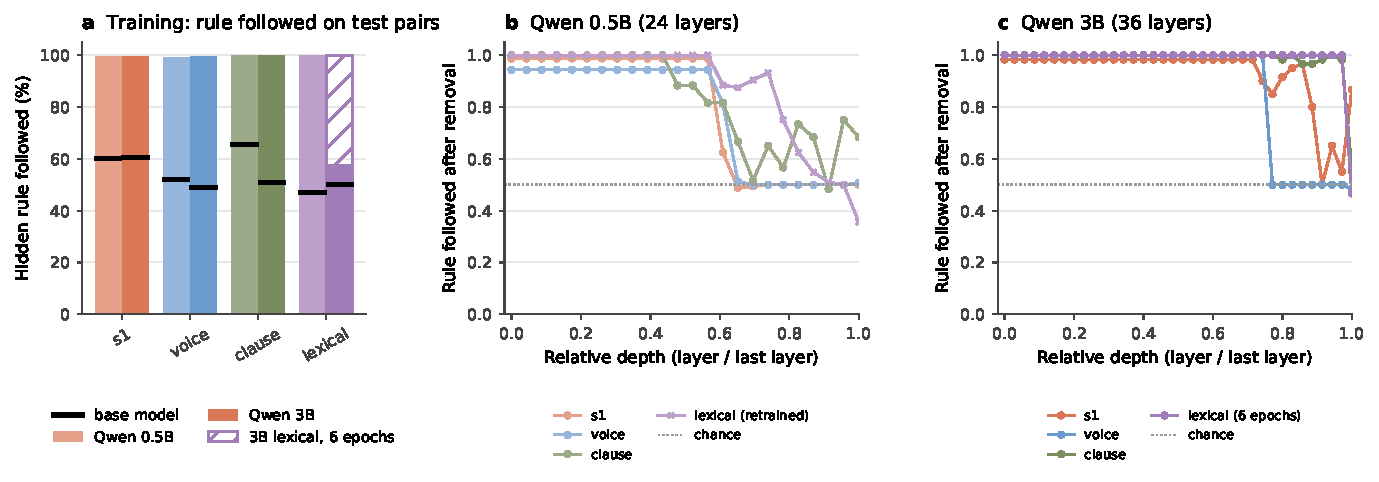
\includegraphics[width=\linewidth]{lab_book/compare_05b_3b.pdf}
\caption{\textbf{Training and depth.} (a) Held-out rule-following for Qwen 0.5B (light) and 3B (dark); black bars are base models. (b, c) Rule-following after removing each rule's own direction at each layer, by relative depth. In 0.5B, s1 and voice drop from about 60\% depth and clause partly from about 45\%; in 3B no rule changes before layer 26 of 36. 0.5B lexical uses the retrained adapter.}
\label{fig:train}
\end{figure}

\subsection{Where can a rule be removed?}

Fig.~\ref{fig:layers} shows both metrics for every layer of Qwen 3B. Random directions never change \dm{} (0.98 at every layer) or \xm. The rules differ:
\begin{itemize}
\item \textbf{Clause} is removed only at the last layer, L35 (\dm{} 0.49, base 0.48); at L27--34 \dm{} stays at 0.94--0.98.
\item \textbf{Voice} is partly removed from L27 (\xm{} 0.50, \dm{} 0.71--0.88) and fully at L35 (\dm{} 0.52).
\item \textbf{s1} shows the clearest collapse: at L32--34 \xm{} falls to 0.51--0.60 but \dm{} stays at 0.98, so the cue is intact and the model just answers 0 (4\% of answers are 1 at L34).
\item \textbf{Lexical} cannot be removed at layers 0--34 (\xm{} $\geq0.96$, \dm{} $\geq0.95$); at L35 \dm{} is 0.48 (base 0.50) with 92\% base preservation. The 6- and 10-epoch adapters give the same profile (Fig.~\ref{fig:lex}).
\end{itemize}
In Qwen 0.5B the retrained lexical adapter starts to weaken at L14 (\dm{} 0.91) and is removed from L19 (\dm{} 0.51--0.57, base 0.49), but at a cost of 14--19\% of base answers. In GPT-OSS-20B no single-direction removal changes answers at layers 0--22 (83--100\% rule-following kept); only the last layer reduces it (55--73\%), and it also changes 12--37\% of base answers. The larger models therefore keep the channel intact until the very end.

\begin{figure}[!htbp]
\centering
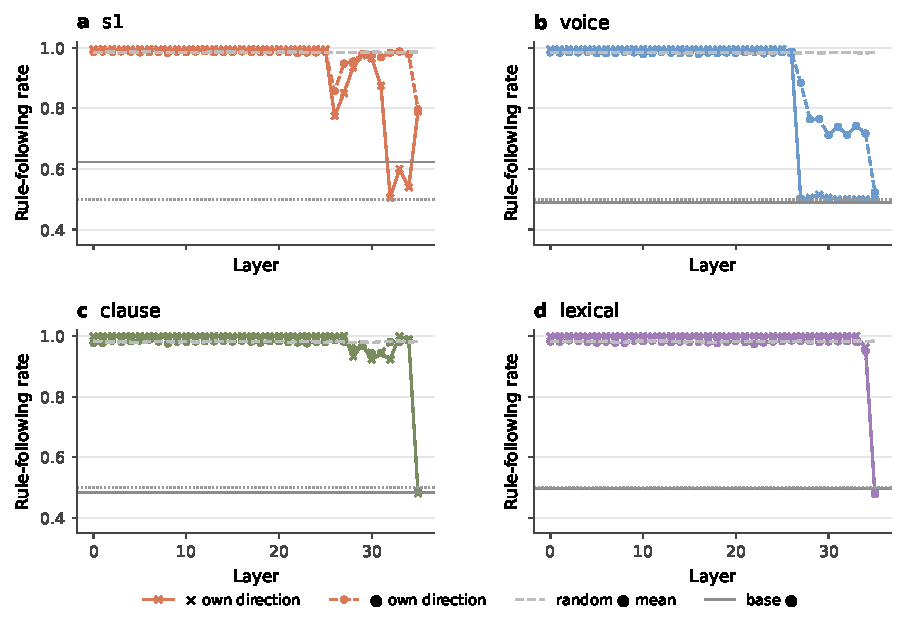
\includegraphics[width=\linewidth]{close_gaps/fig_all_rules_layers.pdf}
\caption{\textbf{Per-layer removal in Qwen 3B.} Rule-following after removing the rule's own direction at each layer: \xm{} (solid) at the model's threshold, \dm{} (dashed) at a cross-fitted threshold. Grey: base model and random-direction mean. Where \xm{} drops but \dm{} stays high (s1, L32--34), the model has collapsed to one label rather than lost the cue.}
\label{fig:layers}
\end{figure}

\begin{figure}[!htbp]
\centering
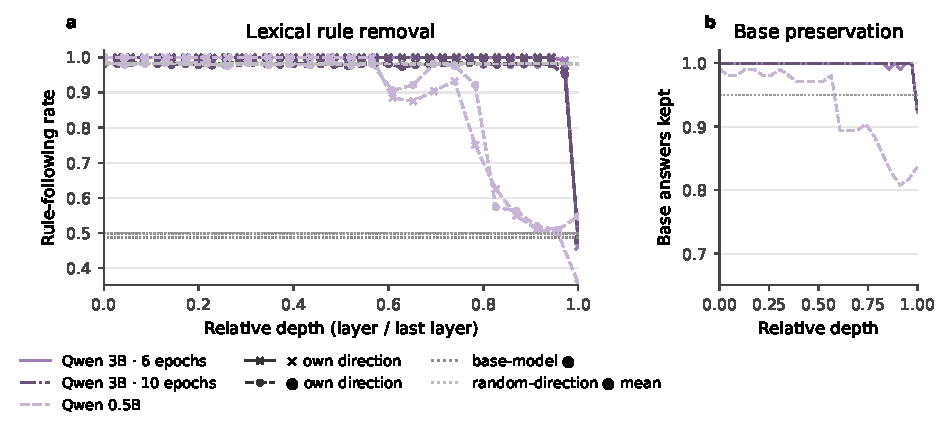
\includegraphics[width=\linewidth]{close_gaps/fig_lexical_layers.pdf}
\caption{\textbf{The lexical rule across layers.} (a) \xm{} and \dm{} after removing the lexical direction, for Qwen 3B (6 and 10 epochs) and Qwen 0.5B, by relative depth. (b) Base preservation. In 3B the rule is removable only at the last layer; in 0.5B from about 80\% depth, with base damage.}
\label{fig:lex}
\end{figure}

At the last layer the residual state reaches the answer only through the unembedding rows for ``0'' and ``1''. Removing a rule direction at L35 therefore works through its overlap with this readout, which every rule shares. Removing a rule direction at L35 also changes many unrelated answers (up to 23\% of base answers for clause). Late removal blocks the path from the rule to the answer; it does not show that the rule was erased.

\subsection{The late common direction is the answer}

The four rules' directions look aligned in late layers: in Qwen 3B their mean cosine is about 0 up to L26 and 0.2--0.35 after, and at L35 kernel probes trained on three rules read the fourth (effect sizes $+2.8$ to $+9.6$). The label-flip control decides what is shared (Fig.~\ref{fig:flip}). On the flipped clause and voice models the same probes give $-4.8$ to $-9.2$: the score reverses in all 8 tests, every held-out pair scores negative, and all tests are significant after Holm correction ($p\le0.007$), also after removing the readout and the base model's answer direction. The shared signal follows the answer, not the cue.

\begin{figure}[!htbp]
\centering
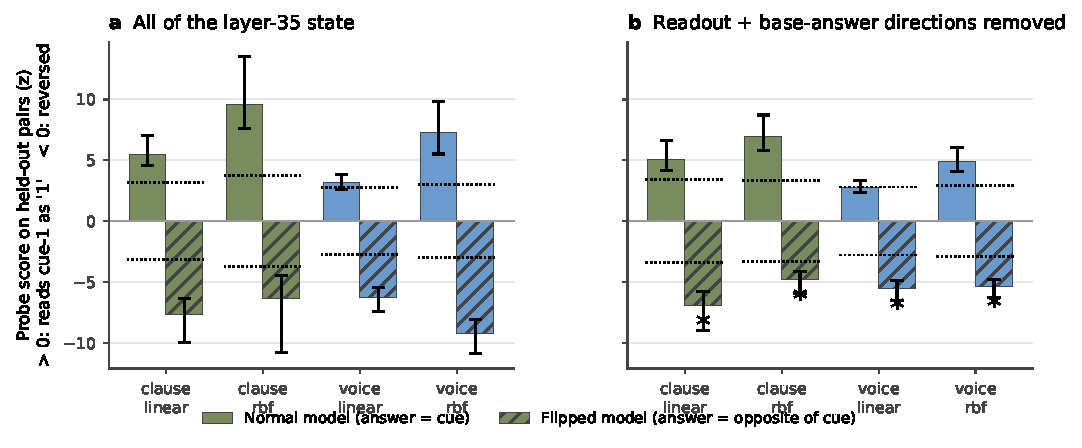
\includegraphics[width=0.85\linewidth]{lab_book/flip.pdf}
\caption{\textbf{Label-flip test at L35.} Probes trained on three normal rules, applied to the held-out rule. Solid: normal adapters (positive = reads the cue). Hatched: flipped adapters, whose answers are reversed. The sign flips in every case, (b) also after removing the readout and base-answer directions: the shared late signal is the answer.}
\label{fig:flip}
\end{figure}

This also explains why all rule arrows sit on one side of a PCA plot. In the original layer-35 PCA axes the normal arrows point to the negative side of PC1, while the flipped clause and voice arrows point to the positive side ($+0.65$, $+0.81$; Fig.~\ref{fig:opp}). The opposite side is not ``anti-steganography''; it is the same cue with the answer reversed.

\begin{figure}[!htbp]
\centering
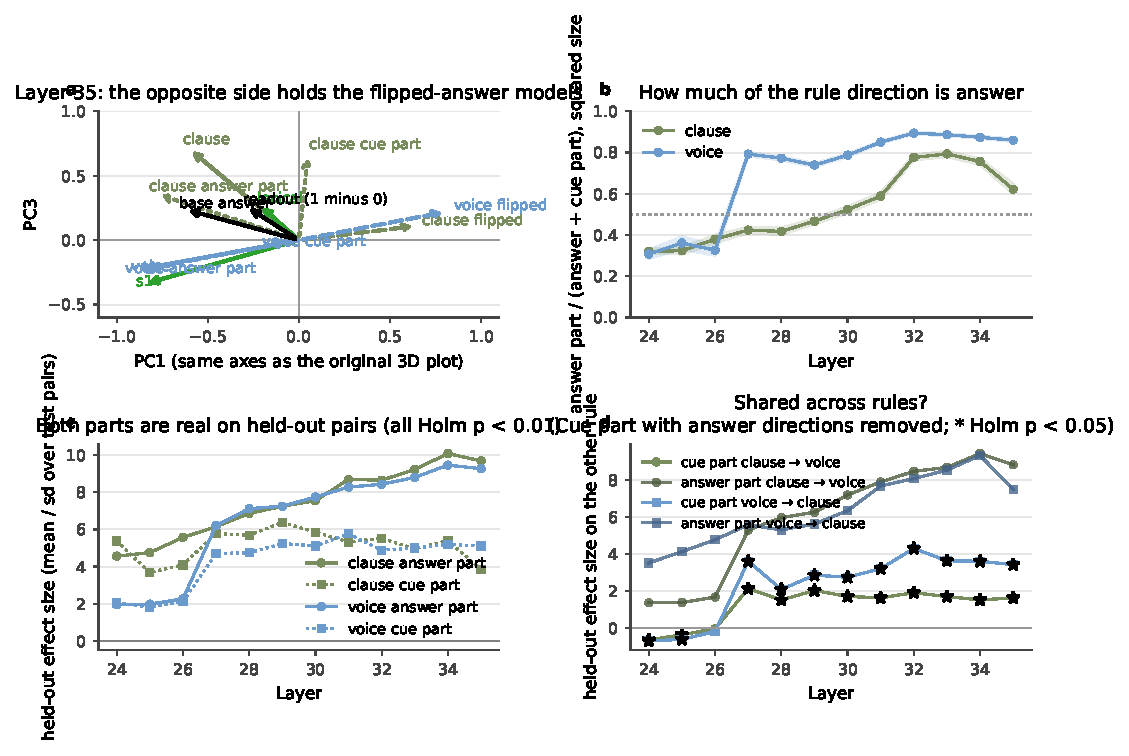
\includegraphics[width=\linewidth]{lab_book/opposite.pdf}
\caption{\textbf{What is on the opposite side?} (a) Normal and flipped arrows in the original PCA axes at L35. Flipped arrows point the other way; their answer parts sit with the normal arrows. (b) Answer part as a share of the arrow by layer. (c, d) Held-out effect sizes of the cue and answer parts, and cue transfer between clause and voice after removing answer directions.}
\label{fig:opp}
\end{figure}

\subsection{Cue and answer at every layer}

We repeat the split at every layer of Qwen 3B for all four rules, with 3 seeds (2 for voice) and matched 10-epoch lexical models. The answer part is under 16\% of every rule direction at layers 0--18. At L35 it is 84--87\% for s1, 86\% for voice, 59--66\% for clause and 31--52\% for lexical (Fig.~\ref{fig:share}). Each rule's cue direction is stable across seeds (cosine 0.5--0.93), but different rules' cue directions are not aligned: cross-rule cosines are near 0 at layers 0--26. From L27, voice--clause reaches 0.29--0.36 and the s1 pairs 0.1--0.2, while lexical stays at $-0.16$ to $0.08$ with every rule. Matching lexical's epochs (10 for both normal and flipped models) does not change this, so lexical's isolation is not an artefact of training length.

\begin{figure}[!htbp]
\centering
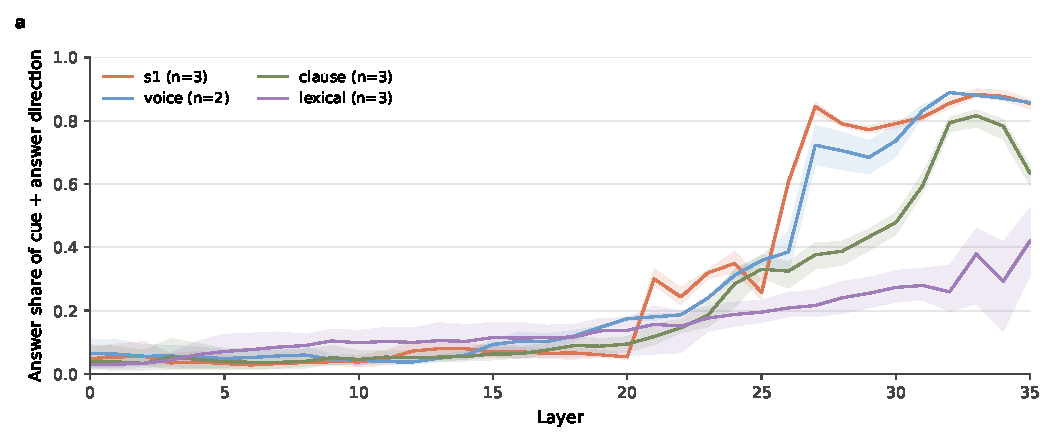
\includegraphics[width=0.49\linewidth]{close_gaps/fig_answer_share.pdf}\hfill
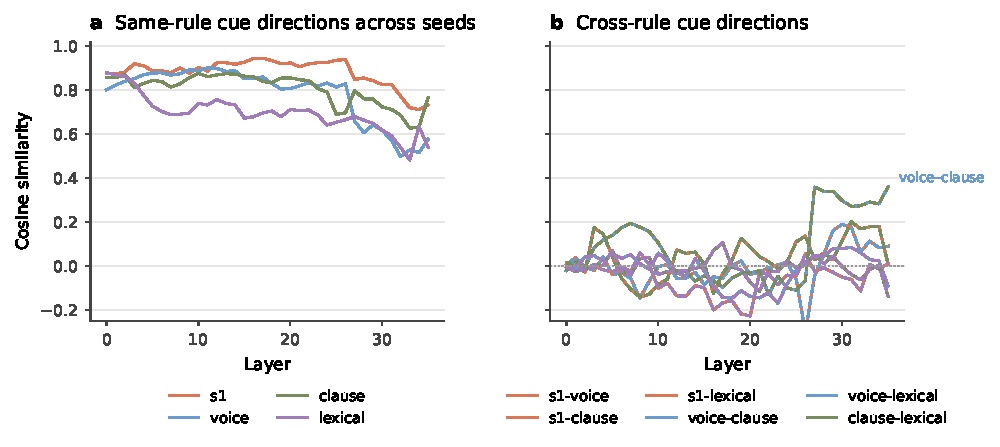
\includegraphics[width=0.49\linewidth]{close_gaps/fig_cue_cosines.pdf}
\caption{\textbf{Cue and answer at every layer (Qwen 3B).} Left: answer share of each rule direction (line = seed mean, band = seed range). Right: cue-direction cosines, the same rule across seeds (ceiling) and between rules. Rules are separate until about 75\% depth; afterwards only voice--clause, and weakly s1, share some cue direction.}
\label{fig:share}
\end{figure}

A more sensitive test projects one rule's held-out cue parts onto another rule's cue direction after removing all answer directions (Fig.~\ref{fig:cue}). For s1, voice and clause this transfer is significant at L27--35 for 16 of 18 rule pairs and layers (Holm $p<0.01$), weak for s1--voice (effect size 0.4--0.8) and stronger for pairs with clause (up to 4.5). Lexical transfers with the opposite sign at L29--35 (0.4--3.8, Holm $p<0.05$). Signs are not comparable across rules, because which variant counts as ``cue 1'' is a per-rule convention; only the size is meaningful.

\begin{figure}[!htbp]
\centering
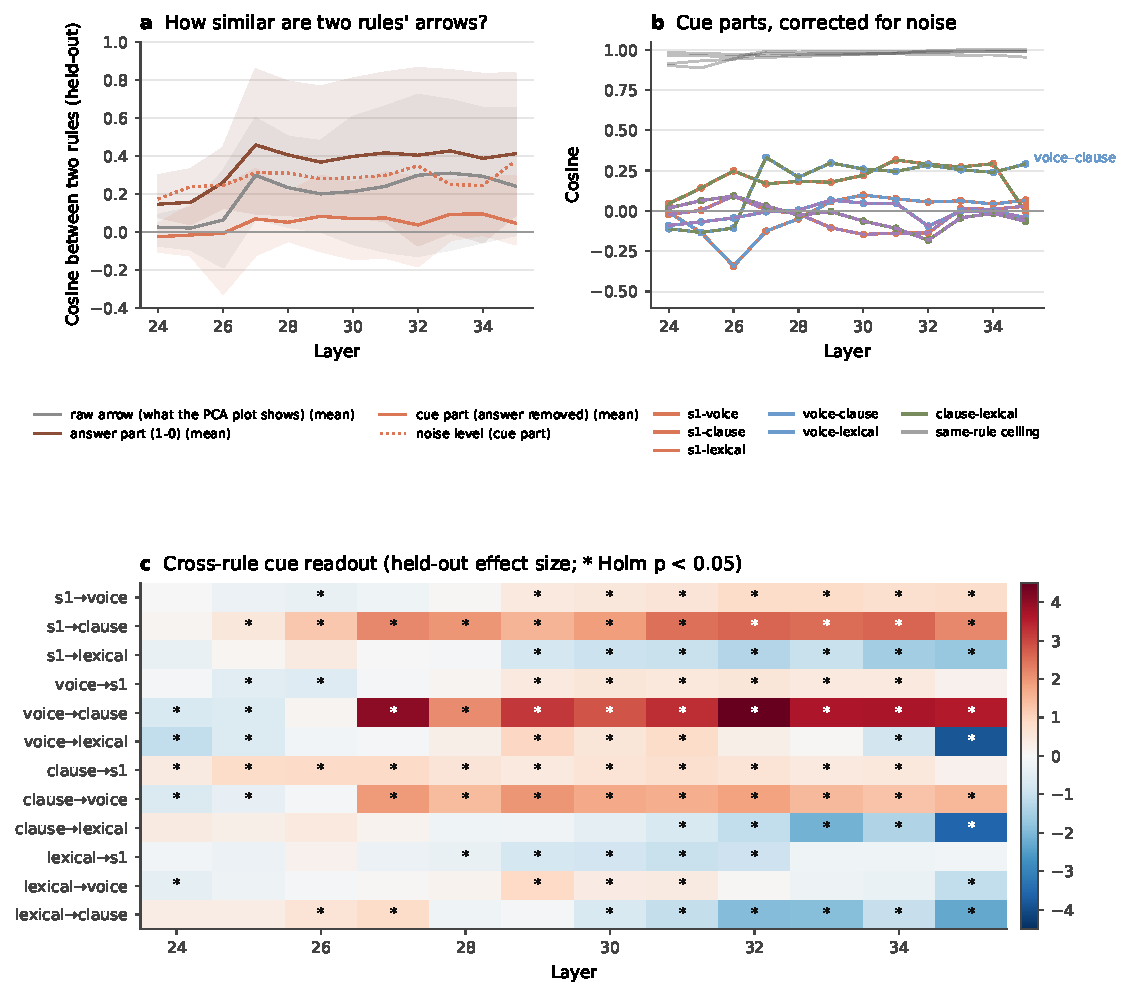
\includegraphics[width=0.92\linewidth]{lab_book/cue_geometry.pdf}
\caption{\textbf{Cue versus answer geometry (seed 0, L24--35).} (a) Cosine between two rules' raw arrows, answer parts and cue parts. The late alignment is in the answer parts. (b) Cross-rule cue cosines with the same-rule ceiling. (c) Held-out cross-rule cue readout effect sizes; $*$ Holm $p<0.05$.}
\label{fig:cue}
\end{figure}

\subsection{Is the shared cue piece used?}

A readable signal need not be used. At L27--30, where later layers could still read it, we removed from each rule's model the span of the other three rules' cue directions (answer directions projected out; rank 3) and compared with 200 random rank-3 subspaces drawn from the same space (Fig.~\ref{fig:shared}). The cue gap (mean margin difference between cue sides) fell by 1--3\% for clause (L27--30), 0.8--1.4\% for voice (L27--28) and 0.3\% for s1 (L27), against at most 0.1\% for random subspaces; lexical did not change. Each of these beats all 200 random subspaces ($p=0.005$), but after Holm correction over the 12 tests run, $p=0.06$. \dm{} stays at 0.98 in every case. Removing the rule's own cue direction at the same layers lowers the gap by 18--36\% for clause but leaves \dm{} at 0.98, and removing its own answer direction lowers the s1 gap by 86--99\% while \dm{} again stays at 0.98: at these depths the cue is stored redundantly and a single subspace does not erase it. The s1 and voice runs at L29--30 did not finish (compute limit).

\begin{figure}[!htbp]
\centering
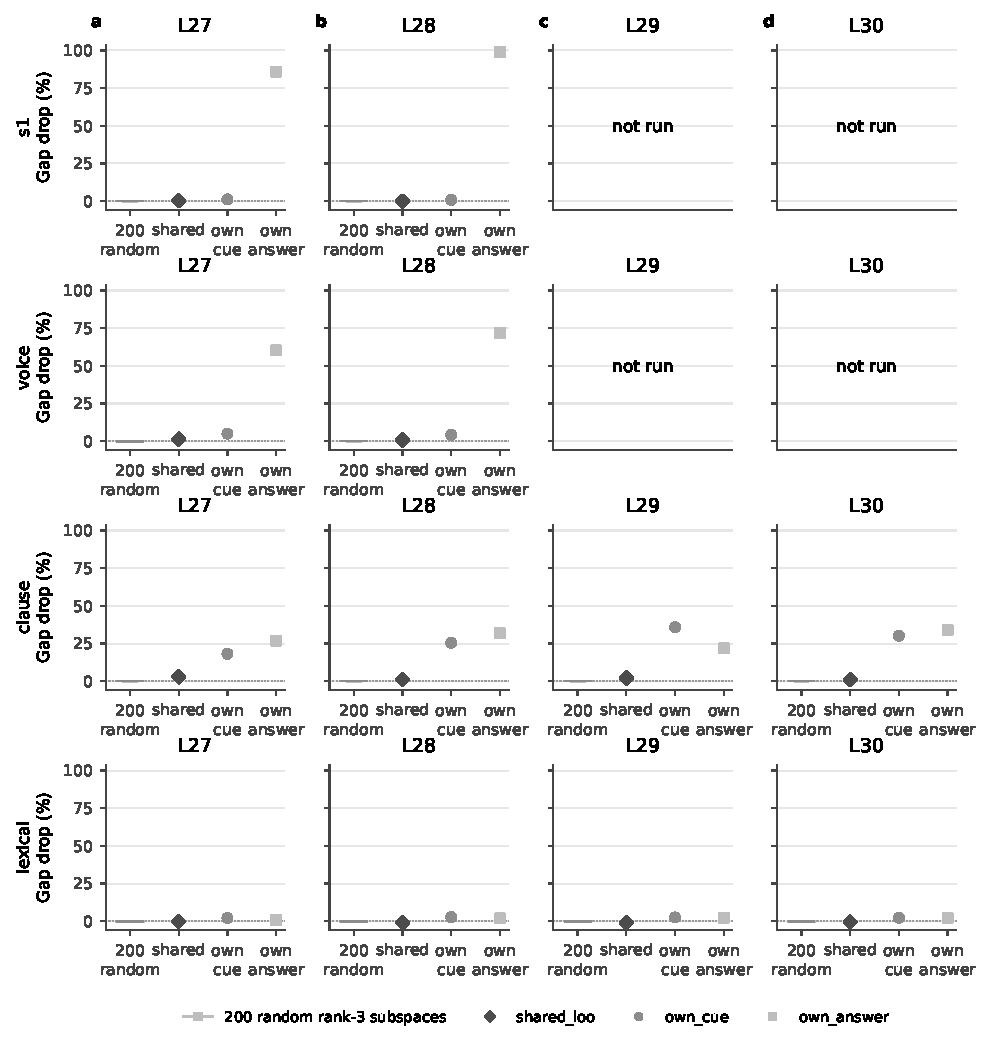
\includegraphics[width=0.8\linewidth]{close_gaps/fig_shared_cue.pdf}
\caption{\textbf{Causal test of the shared cue piece (Qwen 3B, L27--30).} Drop in the cue gap after removing the other rules' cue directions (shared), the rule's own cue or own answer direction. (a) Full scale. (b) Zoom: shared versus the 95th percentile and maximum of 200 random subspaces.}
\label{fig:shared}
\end{figure}

\subsection{The same pattern across models}

Because the models have different widths, we compare the angles between each model's rule directions at the same relative depth (Fig.~\ref{fig:models}). In all three models the four rule directions are unrelated through about the first 75\% of layers (mean cosine inside a sign-flip noise band) and become aligned in the last quarter (0.2--0.35): from L27 in Qwen 3B and from L19 in GPT-OSS; Qwen 0.5B at L18 gives 0.29. Which rules pair up differs: s1--voice at the last layer of Qwen 3B (0.66), s1--lexical in GPT-OSS (0.58). For Qwen 3B the late alignment is shown to be the answer; for GPT-OSS this is likely but untested, since we did not train a flipped GPT-OSS model.

\begin{figure}[!htbp]
\centering
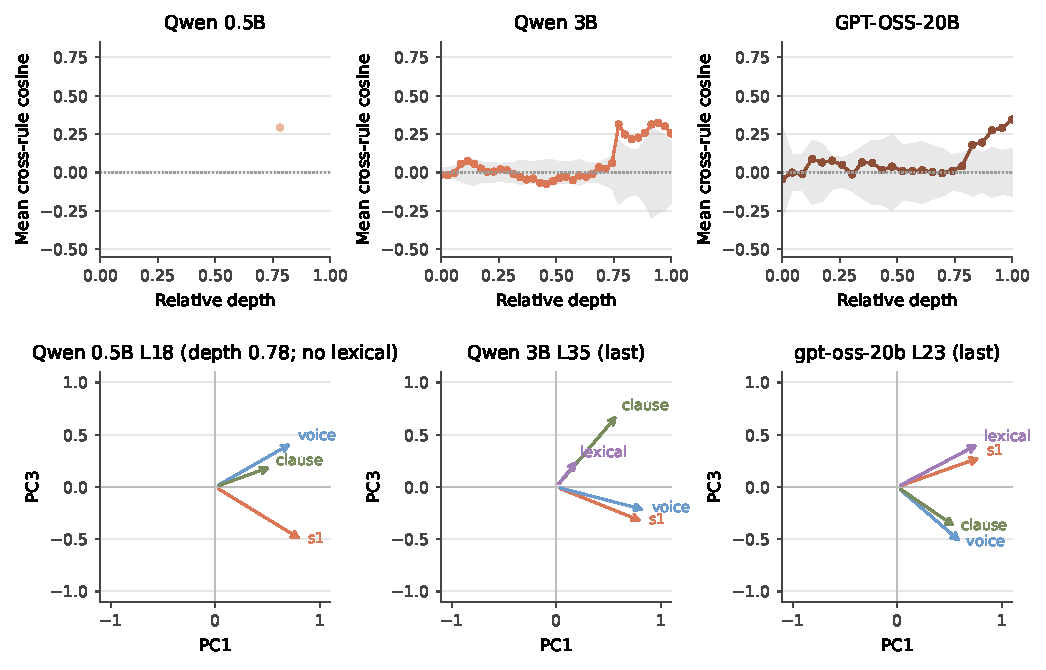
\includegraphics[width=\linewidth]{lab_book/geometry_3models.pdf}
\caption{\textbf{Three models.} (a--c) Mean cosine between rule directions by relative depth, with a noise band. (d--f) Each model's own PCA of its rule directions at a late layer.}
\label{fig:models}
\end{figure}

\section{Discussion}

The results fit one picture. Each hidden rule is first picked up in its own direction; at mid depth these directions are unrelated, consistent with rules at different linguistic levels. In the last quarter of the network the rules converge on a shared 1--0 answer signal, which is what makes them look like one common steganographic code. Once the answer is split off, only a small cue overlap remains, mainly between the two syntactic rules (voice and clause), and the model barely relies on it. The lexical rule is the most isolated: it shares neither cue nor answer direction with the others and is removable only at the final layer in Qwen 3B.

For detection and mitigation this cuts both ways. A probe or ablation that targets the late common direction will appear to work across rules, but it acts on the answer, not on the hidden channel, and in many cases it only collapses the model to one label. Claims of ``removing'' a steganographic behaviour should therefore report a threshold-free measure such as \dm{} and a label-flip control, not only the change in answers. Conversely, the absence of a shared cue direction suggests that a monitor for one encoding will not automatically cover another.

\paragraph{Limitations.} Our data are synthetic, from a single ethics domain, and the message is one bit. Most mechanistic results are for Qwen 3B; the cue/answer split uses 2--3 seeds, but the layer-35 probe tests and the causal test use seed 0 only. Two seeds failed to learn (voice and lexical seed 1). The original 0.5B voice, clause and lexical adapters were lost and the 0.5B lexical analysis uses a retrained adapter. Ablations are rank-1 or rank-3 and at one layer; multi-layer or nonlinear erasure could behave differently. GPT-OSS has no flipped model and no \dm{} analysis yet, and free-generation drops were not checked with \dm. Earlier sparse-autoencoder analyses were trained on too few activations to support claims and are not reported here.

\paragraph{Future work.} Testing lower poisoning rates (30\%, 20\%, 10\% of training data), channels between two models rather than within one, other encodings and families, and sparse dictionaries trained at scale on the label-flip cue parts.

\section{Conclusion}

We built linguistic steganographic channels at three linguistic levels in three models and traced them through the residual stream. The channels are learned easily, stored in separate directions, and removable only late. Their apparent common direction is the shared answer, not a shared code, and a label-flip decomposition makes that distinction measurable. Changing a model's answer is not the same as removing its hidden rule.

\paragraph{Code and data.} Adapters, activations, scans and analysis code:\\ \url{https://github.com/vladflorinfilip/scam} (branch \texttt{close-gaps}).

\renewcommand{\bibfont}{\small}\setlength{\bibsep}{2pt}
\bibliographystyle{abbrvnat}
\bibliography{references}
\end{document}
